This dissertation presents numerous algorithms which aid in identifying safe rooftop landing sites in cities. However, many of our methods are general and can be applied to other domains. In particular, our Polylidar3D algorithm has applications to any problem domain that requires polygon extraction from 2D or 3D data. Such problems readily arise in fields such as computational geometry, \ac{GIS}, and robotics. We have released the open-source software implementations of Polylidar3D and its supporting software under the permissive MIT license \cite{saltzer_origin_2020}. We have carefully optimized each software implementation and tested on both Windows and Linux platforms. All software is hosted online using GitHub, a software development and version control website. Our software is currently being used by academic researchers, software engineers, and geographic information system scientists.  The three main software repositories of interest are:

\begin{enumerate}
    \item Polylidar3D - Fast polygon extraction from 2D and 3D data. \\ Hosted at: \url{https://github.com/JeremyBYU/polylidar}
    \item Fast Gaussian Accumulator (FastGA) - Dominant plane normal estimation for 3D scenes. \\  Hosted at: \url{https://github.com/JeremyBYU/FastGaussianAccumulator}
    \item Organized Point Filters (OPF) - Fast smoothing for organized 3D point clouds.
    \\  Hosted at: \url{https://github.com/JeremyBYU/OrganizedPointFilters}
\end{enumerate}

Each software repository is written in C++ for high performance but includes bindings to Python. We utilize CPU parallelism if available. The build system uses \texttt{CMake} and is tested with the \texttt{msvc} and \texttt{gcc} compilers. Each repository provides documentation through examples as well as the application programming interface (API). Bug reports may be filed at each individual repository. Each section below will provide multi-page screenshots of their respective source code repositories. The screenshots are of the \texttt{README.md} file which provides a summary of the software.

\newpage

%%%%%%%%%%%%%%%%%%%%%%%%%%%%%%%%
%%%%%%%%%%%%%%%%%%%%%%%%%%%%%%%%

% This inserts multi0page snapshots of my repositories as FIGURES.

\section{Polylidar3D Source Code Summary} 
Below is a multi-page screenshot of the \texttt{README.md} file for the Polylidar3D source code repository hosted at \url{https://github.com/JeremyBYU/polylidar}

\begin{figure}[h!]
    \centering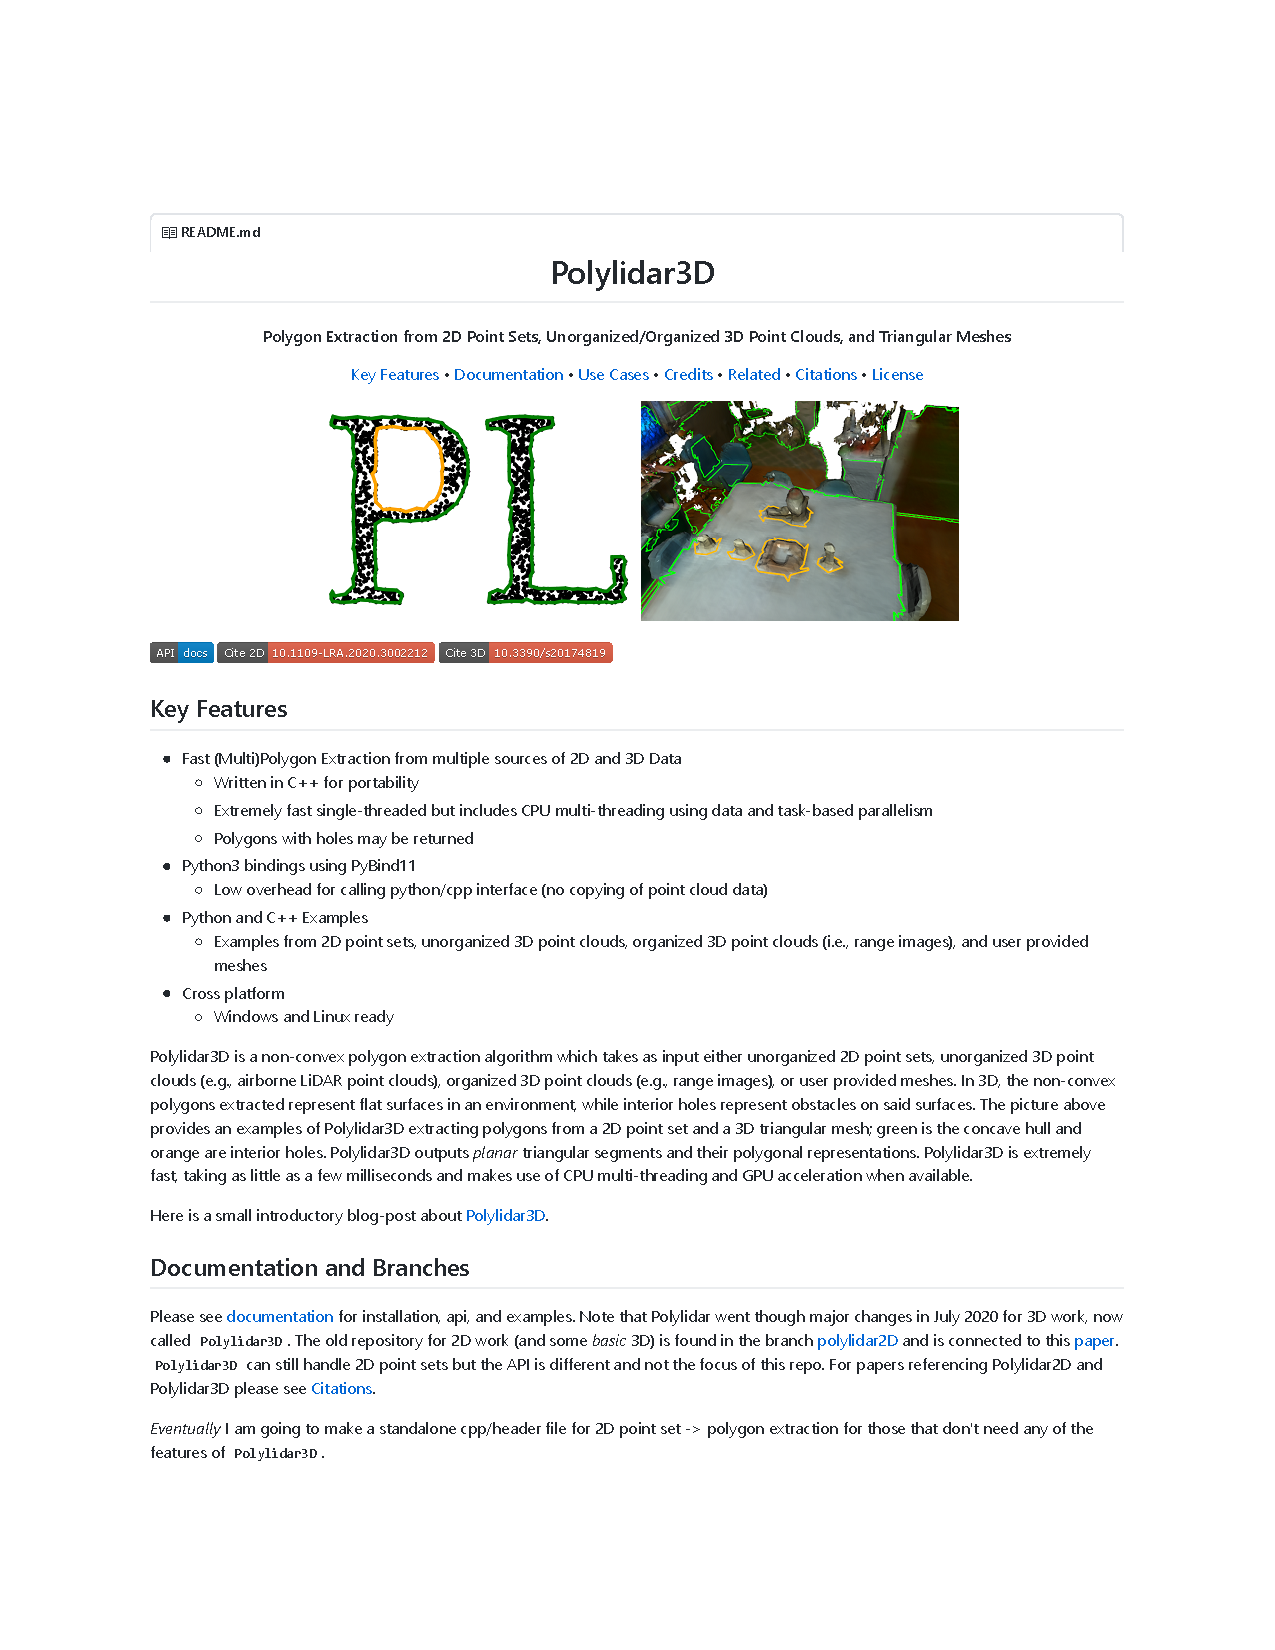
\includegraphics[page=1, trim=1.2in 1.2in 1.2in 1.2in, width=.82\linewidth]{appendix_1/imgs/Polylidar3DReadme.pdf}
    \label{fig:apx1_pl1}
    \caption{Page 1 of the Polylidar3D repository} 
\end{figure}

\begin{figure}[h!]
    \centering\includegraphics[page=2, trim=1.0in 1.0in 1.0in 1.0in, width=.93\linewidth]{appendix_1/imgs/Polylidar3DReadme.pdf}
    \label{fig:apx1_pl2}
    \caption{Page 2 of the Polylidar3D repository} 
\end{figure}

\begin{figure}[h!]
    \centering\includegraphics[page=3, trim=1.0in 1.0in 1.0in 1.0in, width=.93\linewidth]{appendix_1/imgs/Polylidar3DReadme.pdf}
    \label{fig:apx1_pl3}
    \caption{Page 3 of the Polylidar3D repository} 
\end{figure}

\newpage

\section{Fast Gaussian Accumulator Source Code Summary} 
Below is a multi-page screenshot of the \texttt{README.md} file for the FastGA source code repository hosted at \url{https://github.com/JeremyBYU/FastGaussianAccumulator}.

\begin{figure}[h!]
    \centering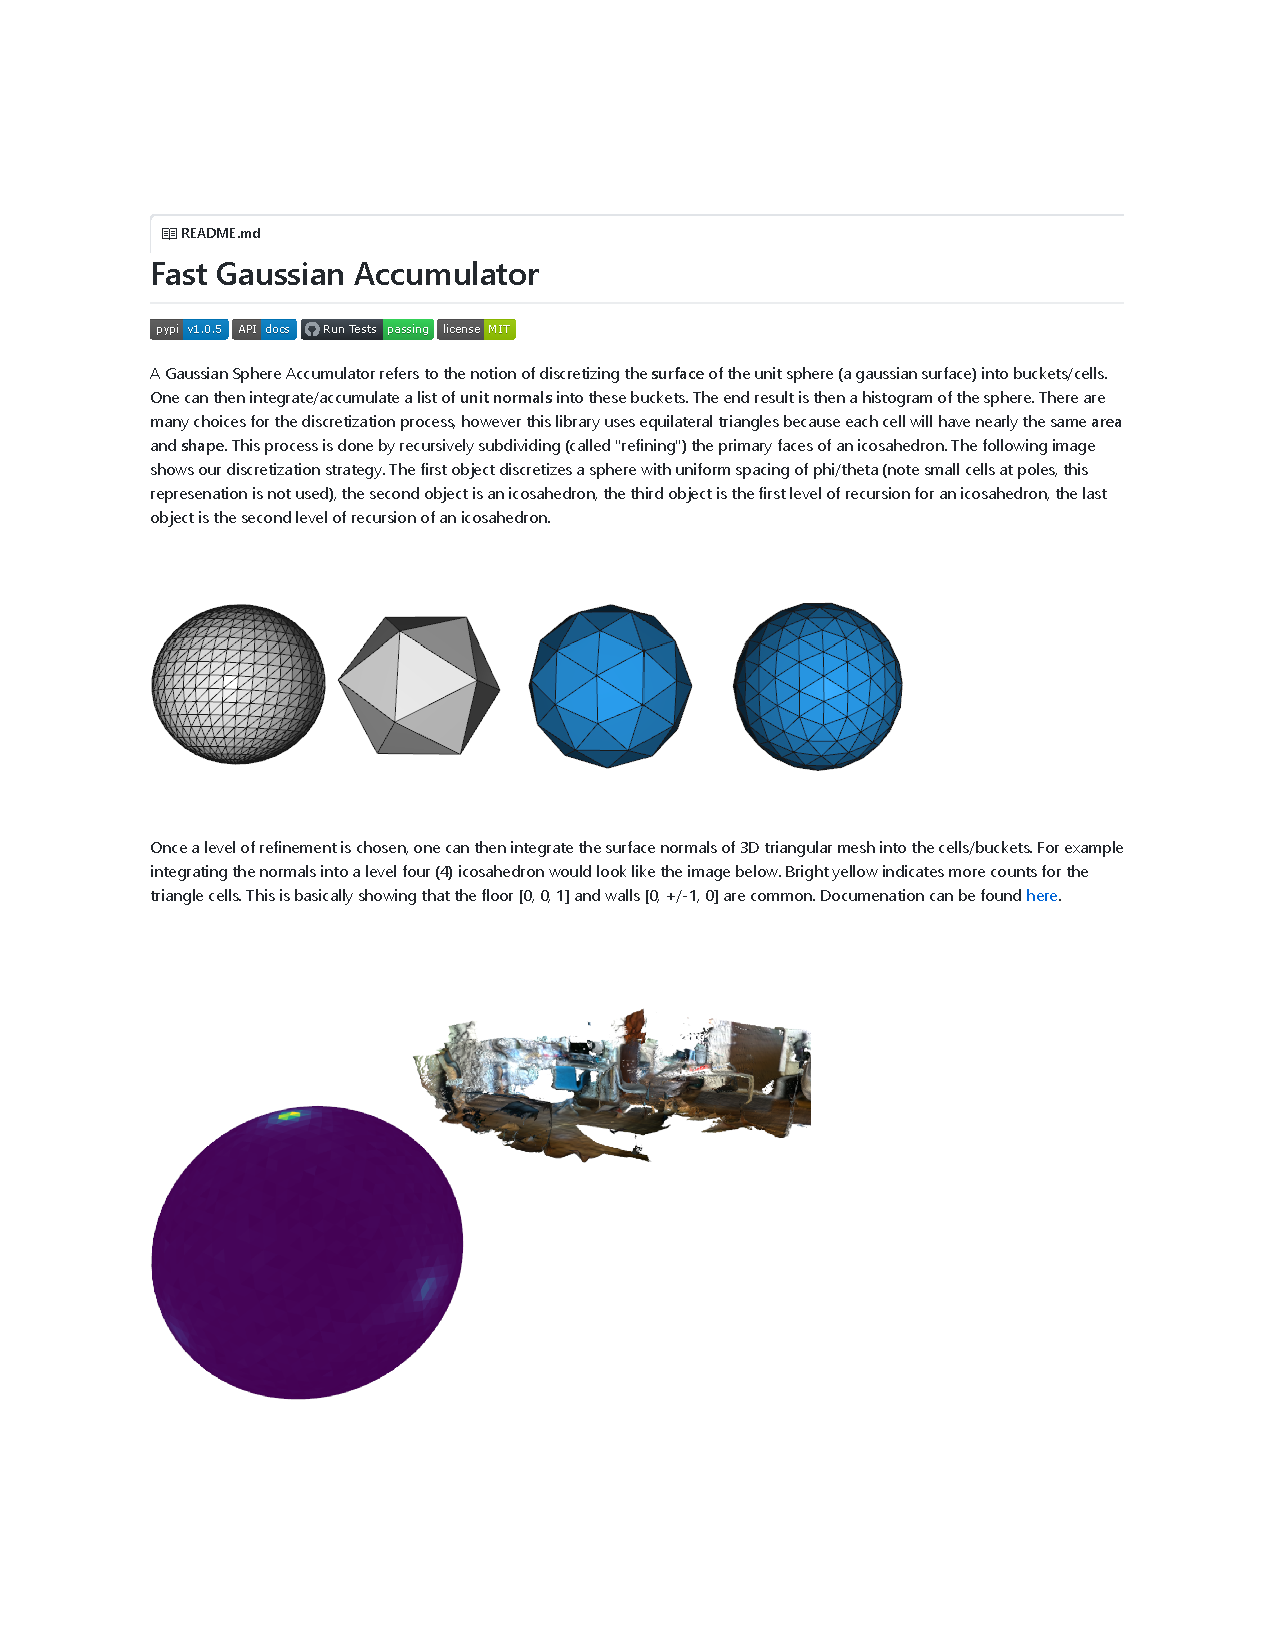
\includegraphics[page=1, trim=1.2in 1.2in 1.2in 1.15in, width=.82\linewidth]{appendix_1/imgs/FastGAReadme.pdf}
    \label{fig:apx1_fg1}
    \caption{Page 1 of the Fast Gaussian Accumulator repository} 
\end{figure}

\begin{figure}[h!]
    \centering\includegraphics[page=2, trim=1.0in 1.0in 1.0in 1.0in, width=.93\linewidth]{appendix_1/imgs/FastGAReadme.pdf}
    \label{fig:apx1_fg2}
    \caption{Page 2 of the Fast Gaussian Accumulator repository} 
\end{figure}

\begin{figure}[h!]
    \centering\includegraphics[page=3, trim=1.0in 1.0in 1.0in 1.0in, width=.93\linewidth]{appendix_1/imgs/FastGAReadme.pdf}
    \label{fig:apx1_fg3}
    \caption{Page 3 of the Fast Gaussian Accumulator repository} 
\end{figure}

\newpage

\section{Organized Point Filters Source Code Summary} 
Below is a multi-page screenshot of the \texttt{README.md} file for the OPF source code repository hosted at \url{https://github.com/JeremyBYU/OrganizedPointFilters}.

\begin{figure}[h!]
    \centering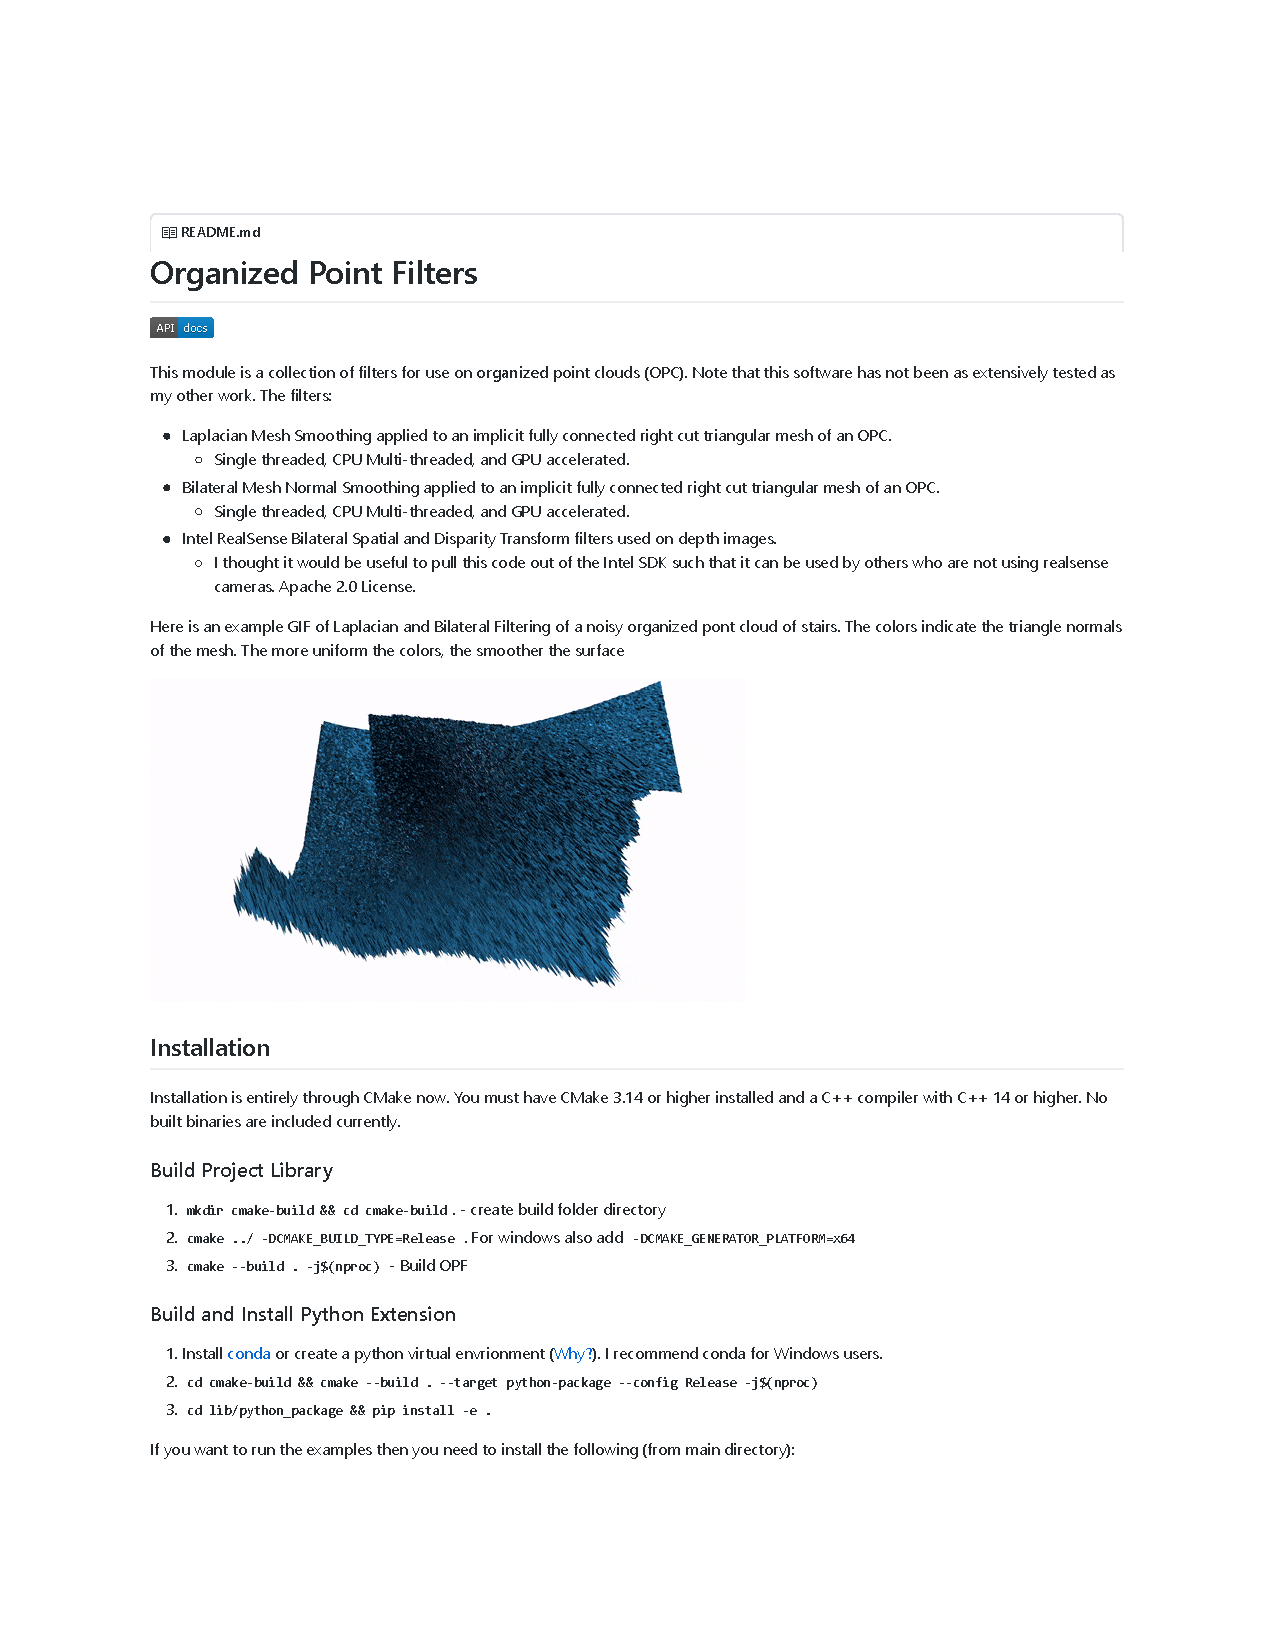
\includegraphics[page=1, trim=1.2in 1.2in 1.2in 1.15in, width=.82\linewidth]{appendix_1/imgs/OPFReadme.pdf}
    \label{fig:apx1_opc1}
    \caption{Page 1 of the Organized Point Filter repository} 
\end{figure}

\begin{figure}[h!]
    \centering\includegraphics[page=2, trim=1.0in 1.0in 1.0in 1.0in, width=.93\linewidth]{appendix_1/imgs/OPFReadme.pdf}
    \label{fig:apx1_opc2}
    \caption{Page 2 of the Organized Point Filter repository} 
\end{figure}

%%%%%%%%%%%%%%%%%%%%%%%%%%%%%%%%
%%%%%%%%%%%%%%%%%%%%%%%%%%%%%%%%

% Below uses the \includepdf method. I prefer this but not sure if Rackham will allow. Sad Face....

% 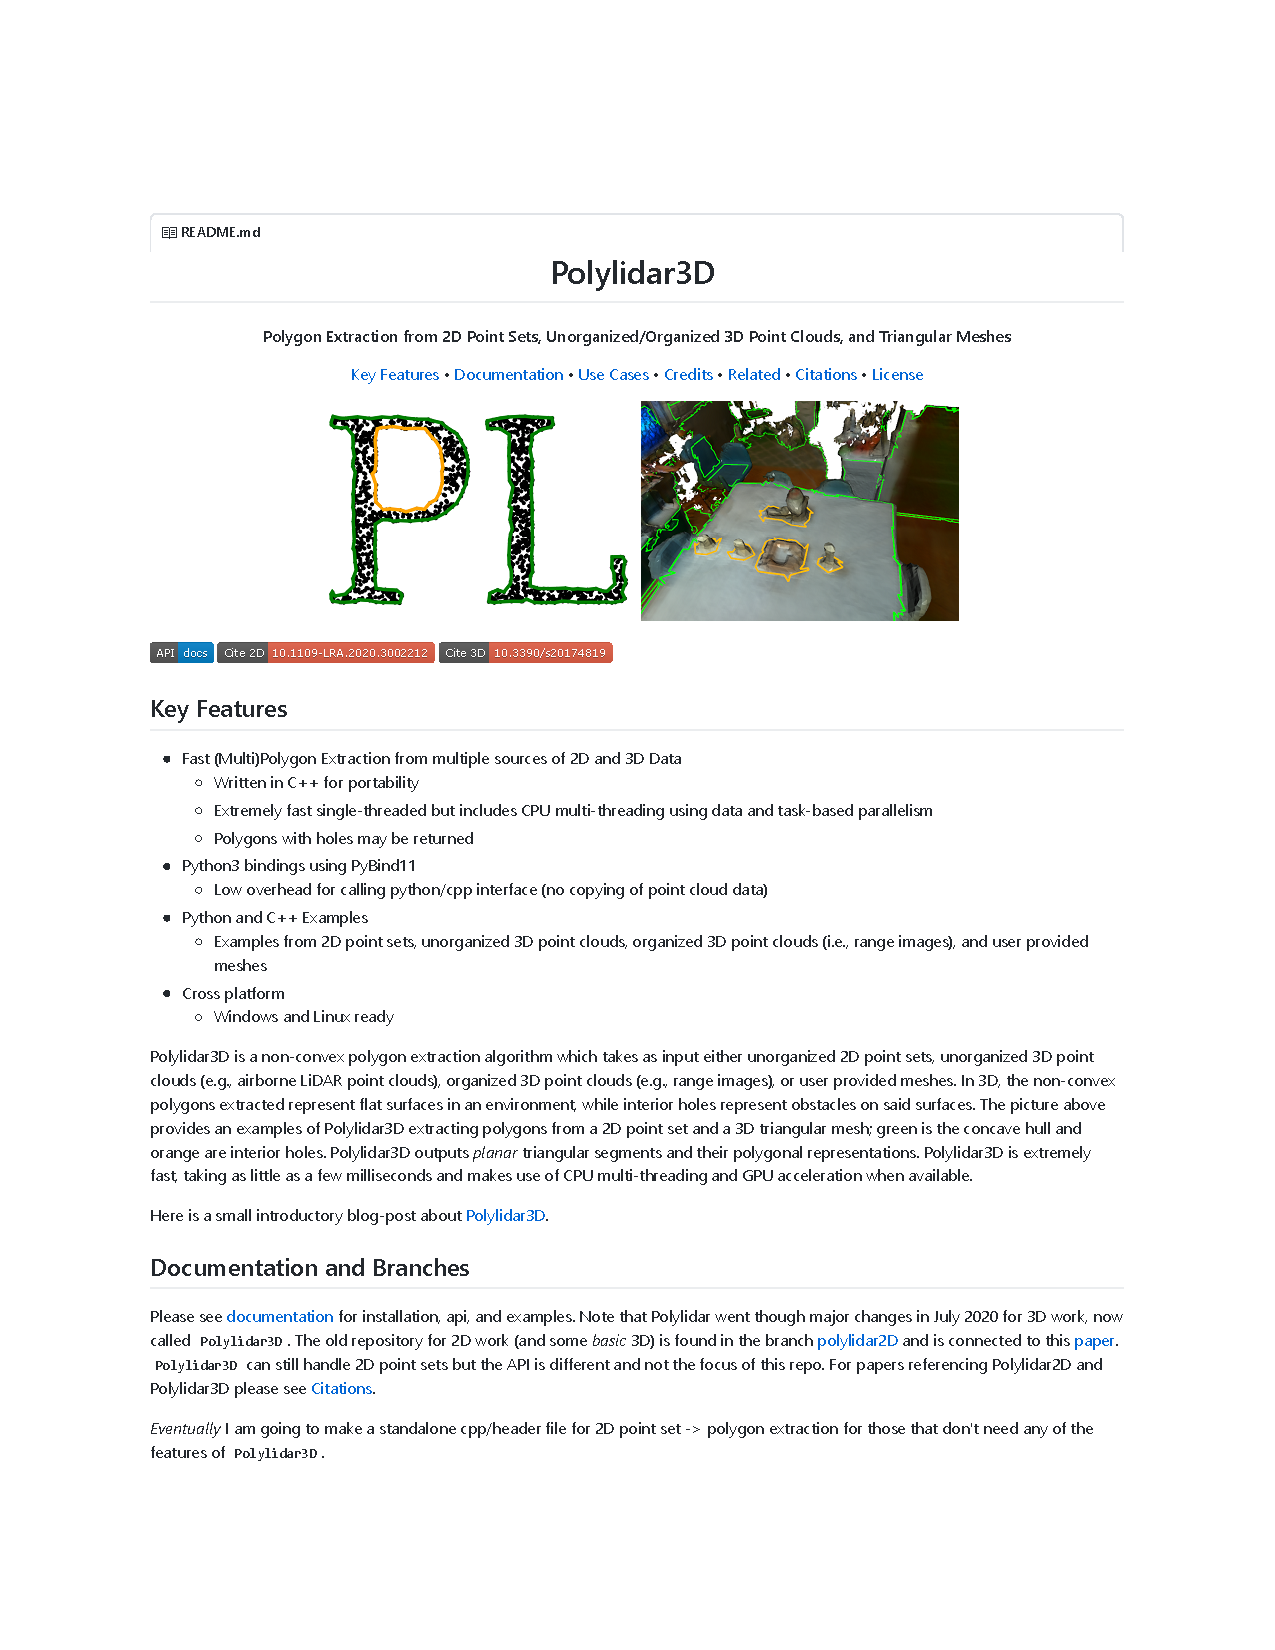
\includepdf[pages=1,pagecommand={\section{Polylidar3D Source Code Summary} Below is a multi-page screenshot of the \texttt{README.md} file for the Polylidar3D source code repository hosted at \url{https://github.com/JeremyBYU/polylidar}. {}}, fitpaper=false, scale=0.95, offset=0 -1.1cm]{appendix_1/imgs/Polylidar3DReadme.pdf}
% \includepdf[pages=2-,pagecommand={}, fitpaper=true]{appendix_1/imgs/Polylidar3DReadme.pdf}


% 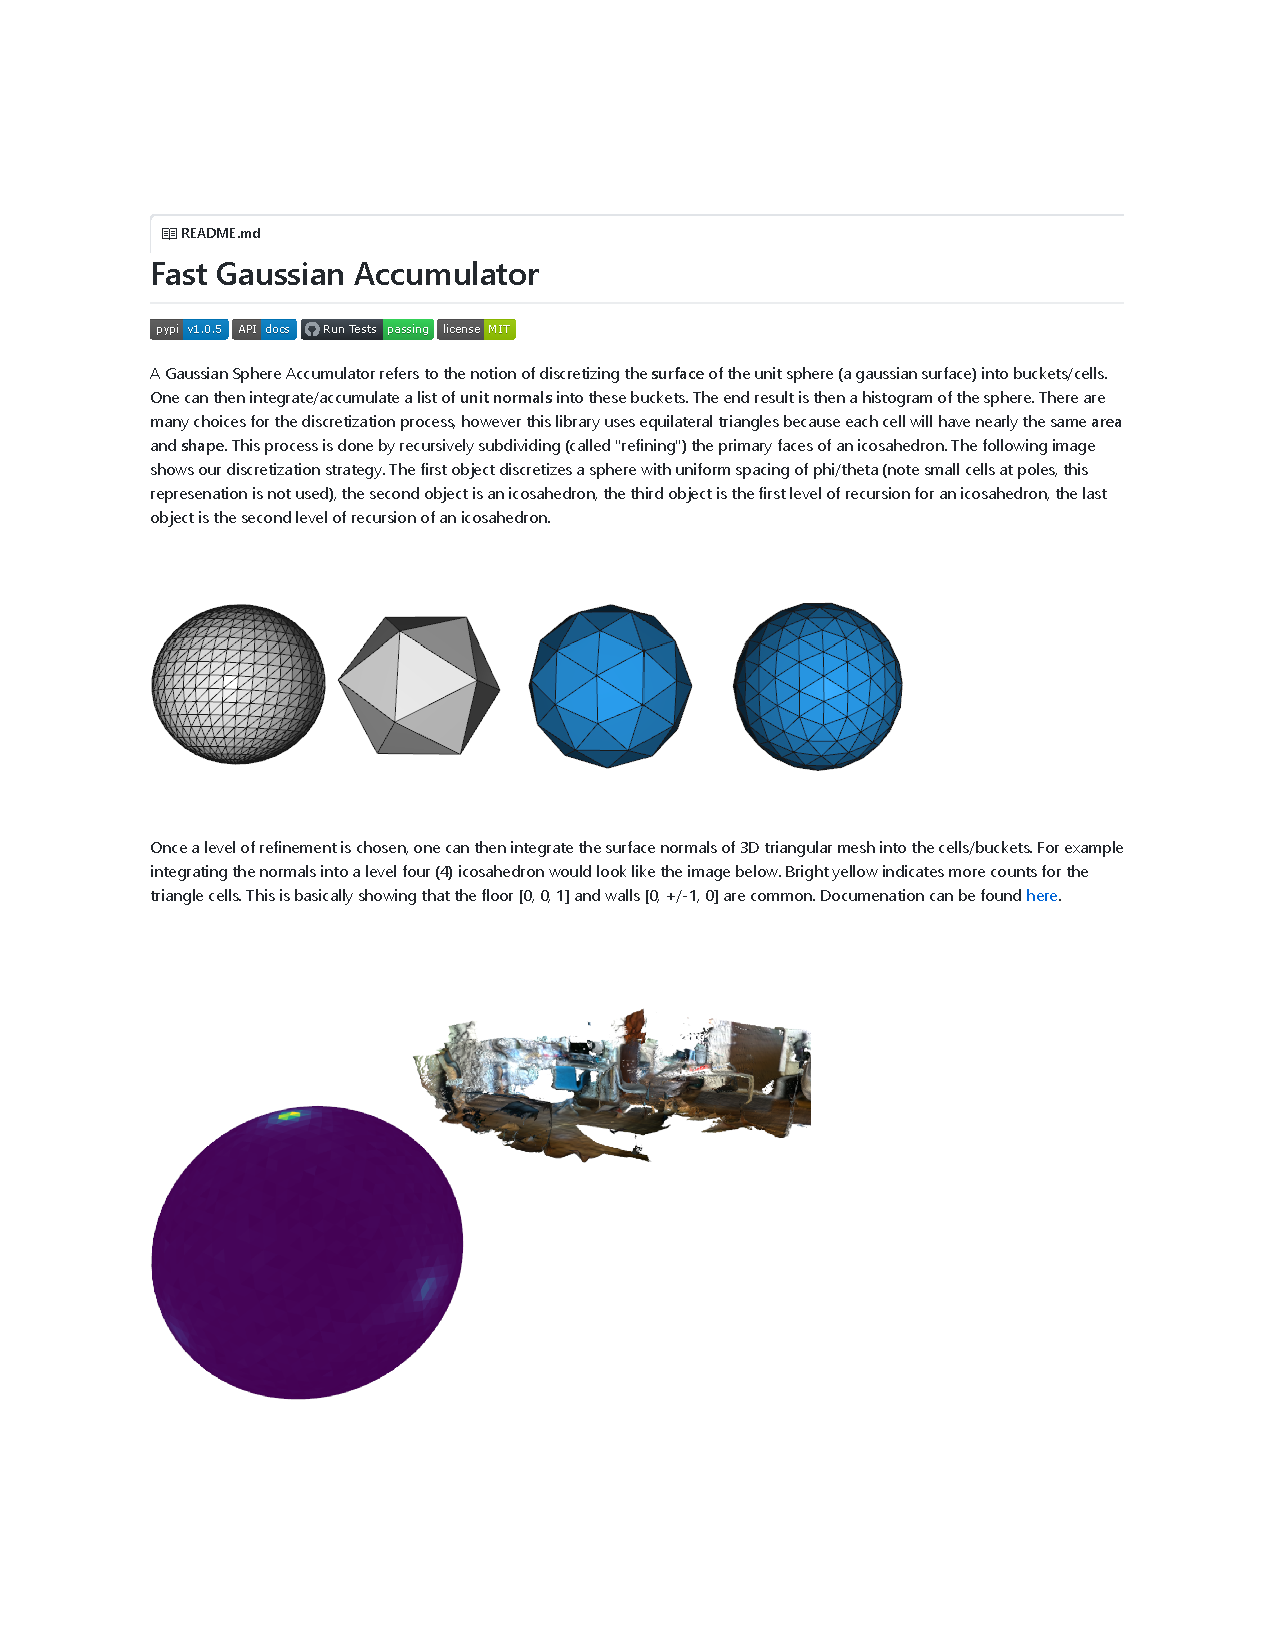
\includepdf[pages=1,pagecommand={\section{Fast Gaussian Accumulator Source Code Summary} Below is a multi-page screenshot of the \texttt{README.md} file for the FastGA source code repository hosted at \url{https://github.com/JeremyBYU/FastGaussianAccumulator}. {}}, fitpaper=false, scale=0.95, offset=0 -1.1cm]{appendix_1/imgs/FastGAReadme.pdf}
% \includepdf[pages=2-,pagecommand={}, fitpaper=true]{appendix_1/imgs/FastGAReadme.pdf}


% 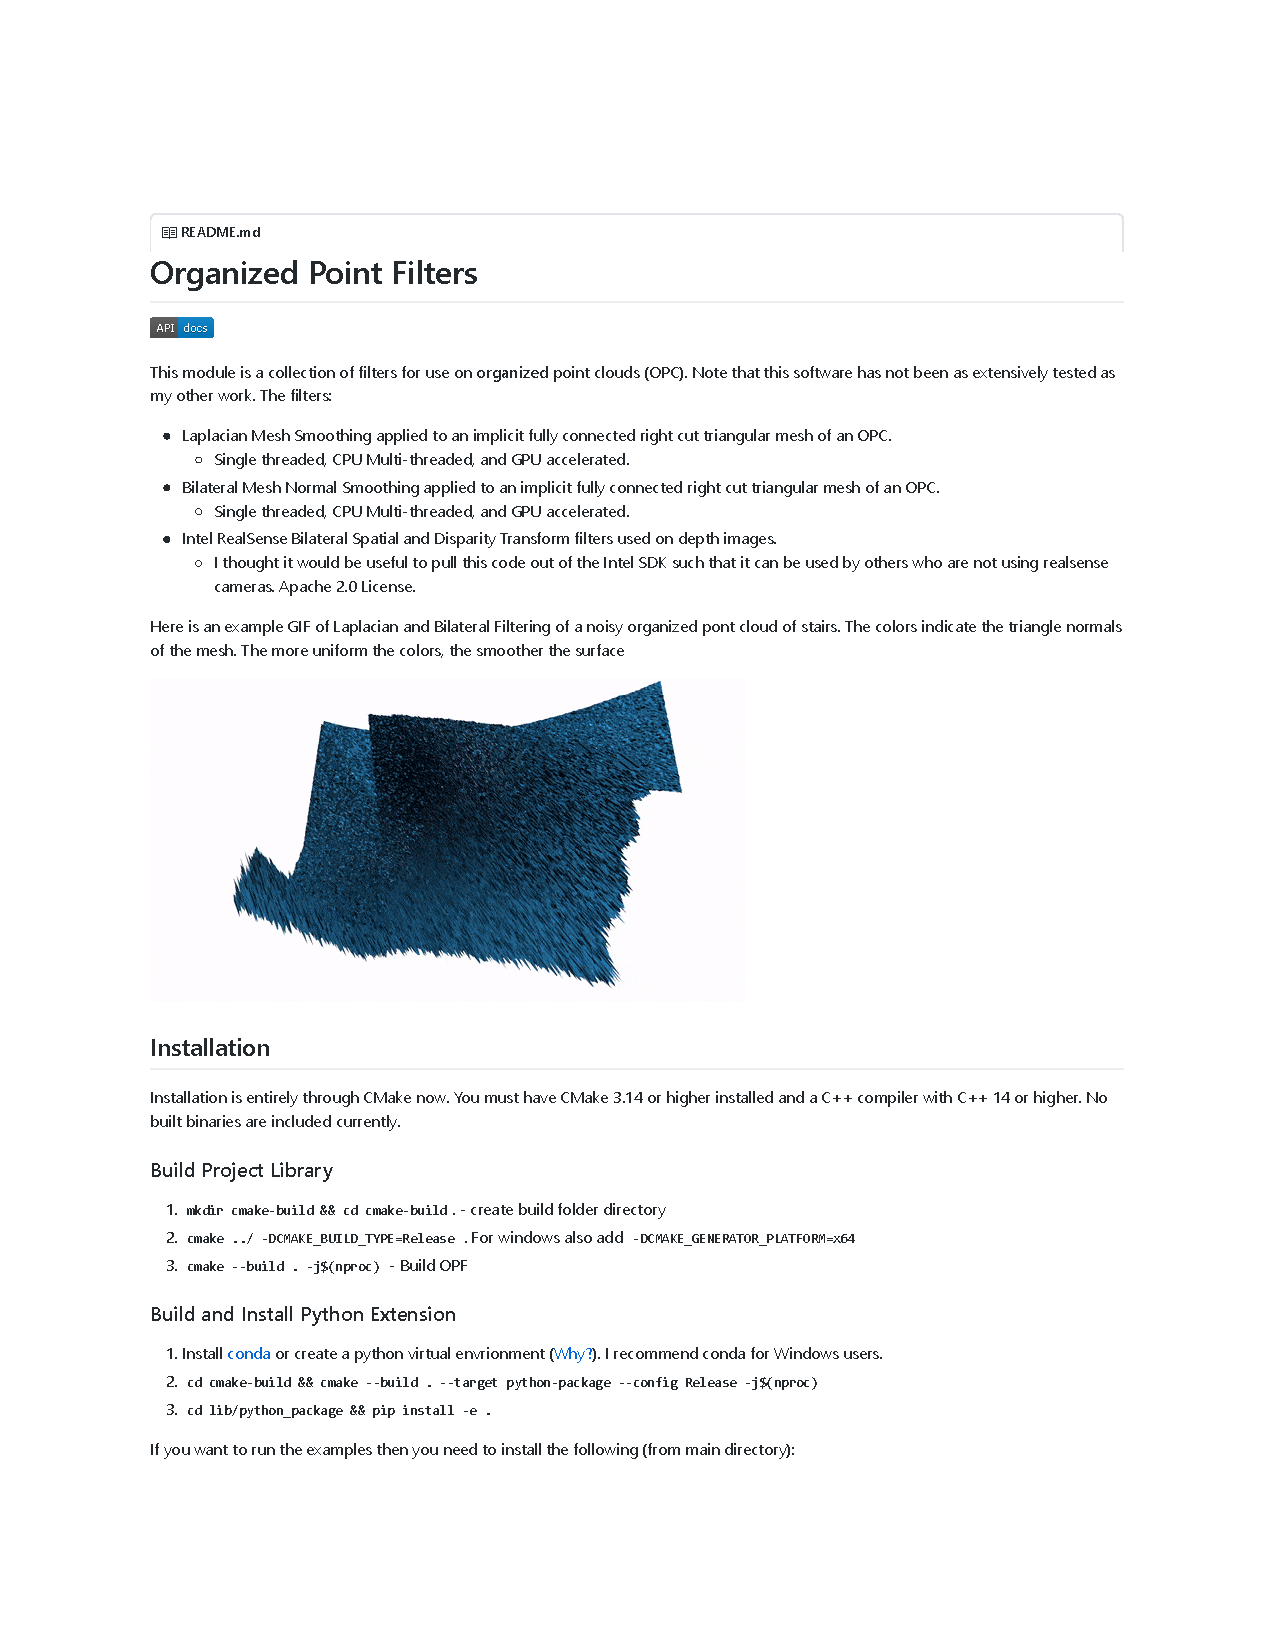
\includepdf[pages=1,pagecommand={\section{Organized Point Filters Source Code Summary} Below is a multi-page screenshot of the \texttt{README.md} file for the OPF source code repository hosted at \url{https://github.com/JeremyBYU/OrganizedPointFilters}. {}}, fitpaper=false, scale=0.95, offset=0 -1.1cm]{appendix_1/imgs/OPFReadme.pdf}
% \includepdf[pages=2,pagecommand={}, fitpaper=true]{appendix_1/imgs/OPFReadme.pdf}


